% Tamaño de letra.
\documentclass[12pt,titlepage]{article}

%------------------------------ Paquetes ----------------------------------

% Paquetes:

%Para comentarios multilínea.
\usepackage{verbatim}

% Para tener cabecera y pie de página con un estilo personalizado.
\usepackage{fancyhdr}

% Codificación UTF-8
\usepackage[utf8]{inputenc}

% Castellano.
\usepackage[spanish]{babel}

% Tamaño de página y márgenes.
\usepackage[a4paper,headheight=16pt,scale={0.75,0.8},hoffset=0.5cm]{geometry}

% Para poder agregar notas al pie en tablas:
%\usepackage{threeparttable}

% Tipo de letra Helvetica (Arial).
%\usepackage{helvet}
%\renewcommand\familydefault{\sfdefault}

% Gráficos:

% Para incluir imágenes, el siguiente código carga el paquete graphicx
% según se esté generando un archivo dvi o un pdf (con pdflatex).

% Para generar dv.
%\usepackage[dvips]{graphicx}

% Para generar pdf.
\usepackage[pdftex]{graphicx}
\pdfcompresslevel=9

\usepackage{appendix}
\usepackage{pdfpages}
\usepackage{longtable}
\usepackage{url}


%
% Directorio donde están las imagenes.
%
%\newcommand{\imgdir}{includes}
%\graphicspath{{\imgdir/}}

%------------------------------ ~paquetes ---------------------------------

%------------------------- Inicio del documento ---------------------------

\begin{document}

% ---------------------- Encabezado y pie de página -----------------------

% Encabezado: sección a la derecha.
% Pie de página: número de página a la derecha.

\pagestyle{fancy}
\renewcommand{\sectionmark}[1]{\markboth{}{\thesection\ \ #1}}
\lhead{}
\chead{}
\rhead{\rightmark}
\lfoot{}
\cfoot{}
\rfoot{\thepage}

% ---------------------- ~Encabezado y pie de página ----------------------

% -------------------------- Título y autor(es) ---------------------------

\title{ConcuShare}
\author{}

% -------------------------- ~Título y autor(es) --------------------------

% ------------------------------- Carátula --------------------------------

\begin{titlepage}

\thispagestyle{empty}

% Logo facultad más pie de la figura.
\begin{center}

\includegraphics[scale=0.55]{./Images/fiuba}\\
\large{\textsc{Universidad de Buenos Aires}}\\
\large{\textsc{Facultad De Ingeniería}}\\
\small{Año 2012 - 1\textsuperscript{er} Cuatrimestre}
\end{center}

\vfill

% Título central.
\begin{center}

\Large{\underline{\textsc{Sistema de Programaci\'on No Convencional de Robots}}}
\Large{\underline{\textsc{(75.70)}}}

\vfill

% Tabla de integrantes.

\Large{\underline{\textsc{Trabajo Pr\'actico}}}

\vfill

\Large\underline{Integrantes} \linebreak\linebreak

% Separación entre columnas.
\large\addtolength{\tabcolsep}{-3pt}
% Tres columnas con alineación centrada.
\begin{tabular}{|| c | c | c ||}
\hline
\textbf{Apellido, Nombre} & \textbf{Nro. Padrón} & \textbf{E-mail} \\
\hline
Bukaczewski, Verónica & 86954 & vero13@gmail.com \\
\hline
Rivero, Hern\'an & XXXXXX & riverohernanj@gmail.com \\
\hline
\end{tabular}
\end{center}

\vfill

\hrule
\vspace{0.2cm}

% Pie de página de la carátula.
%\noindent\small{75.70 - Sistema de Programaci\'on No Convencional de Robots \hfill}

\end{titlepage}

% ------------------------------- ~Carátula -------------------------------

% ----------------------- Cabeceras y pies de página ----------------------

\pagestyle{fancy}
\lhead{}
\chead{}
\rhead{}
\lfoot{\scriptsize{75.70 - Sistema de Programaci\'on No Convencional de Robots \\
\\Trabajo práctico 0 - 1er cuatrimestre 2012}}
\cfoot{}
\rfoot{\\\thepage}
\renewcommand{\headrulewidth}{0pt}

% ---------------------- ~Cabeceras y pies de página ----------------------

% -------------------------------- Índice ---------------------------------

% Hago que las páginas se comiencen a contar a partir de aquí.
\setcounter{page}{2}

% Índice.
\newpage
\thispagestyle{empty}
\tableofcontents
\newpage

% -------------------------------- ~Índice --------------------------------

% ----------------------------- Inicio del tp -----------------------------

\section{Objetivo}
El objetivo del presente trabajo pr\'actico es familiarizarnos con la herramienta Joone, utilizada para el estudio de Redes Neuronales. Y finalmente, poder realizar una an\'alisis de los resultados obtenidos.

\section{Descripci\'on base de datos seleccionada}
Se seleccion\'o la base de datos del TA-TE-TI, extra\'ida de la p\'agina UCI (Machine Learning Repository) \cite{UCI}. Esta base de datos codifica el conjunto completo de configuraciones posibles para el final del juegos del TA-TE-TI, donde "x" se supone que juega primero. El concepto objetivo es "ganar para x" (es decir, ocurre cuando "x" tiene una de las 8 posibles maneras de crear un "tres-en-l\'inea").

\subsection{Informaci\'on relevante}

\begin{itemize}
 \item N\'umero de instancias: 958.
 \item N\'umero de atributos: 10.
 \item Informaci\'on de los atributos: (x=player x has taken, o=player o has taken, b=blank)
    \begin{enumerate}
      \item top-left-square: {x,o,b}
      \item top-middle-square: {x,o,b}
      \item top-right-square: {x,o,b}
      \item middle-left-square: {x,o,b}
      \item middle-middle-square: {x,o,b}
      \item middle-right-square: {x,o,b}
      \item bottom-left-square: {x,o,b}
      \item bottom-middle-square: {x,o,b}
      \item bottom-right-square: {x,o,b}
      \item Class: {positive,negative}
    \end{enumerate}
 \item Falta de valores de atributo: Ninguno.
 \item Distribución de Clase: 65,3\% son positivos (es decir, gana para "x").
\end{itemize}

\section{Preparando los datos para las corridas}
Los valores para los atributos fueron modificados para que el programa Joone pueda ejecutarse correctamente;
debido a que s\'olo trabaja con n\'umeros reales y enteros. \\
{\bf{Valores:}}
    \begin{enumerate}
      \item x= +1
      \item o= -1
      \item b= 0
      \item positive= 1
      \item negative= 0
    \end{enumerate}

\section{Red Neuronal}
Para el armado de la red neural, se tuvo en cuenta que la cantidad de casilleros del tablero de Ta-Te-Ti es 9 y que por cada uno se tiene la posibilidad de encontrar tres tipos de elementos (cruz, c\'irculo y vac\'io). Entonces, como primera capa oculta se decidi\'o utilizar 27 (9x3) filas. Para las siguientes capas ocultas se decidieron utilizar 9 y 3 filas, en funci\'on de la cantidad de casilleros y elementos posibles. \\

Para entrenar la red se requirieron datos que representen el comportamiento deseado. \\
En la base de datos original encontramos diez columnas, las nueve primeras representan los lugares del tablero del Ta-Te-Ti y la \'ultima columna representa si gana el jugador ``x''.

\begin{center}
 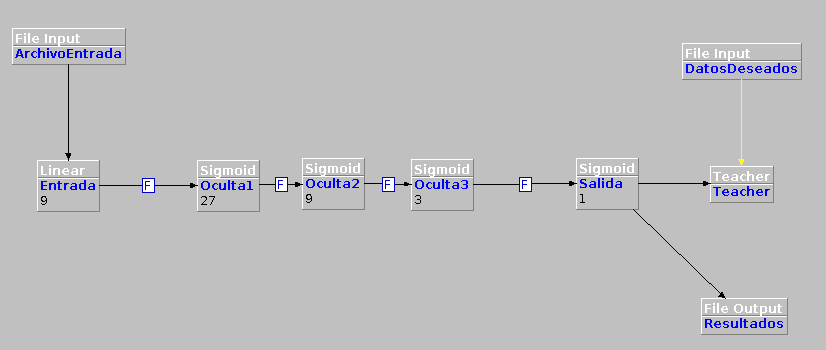
\includegraphics[width=500,height=250]{./Images/RN.png}
 % RN.png: 826x350 pixel, 96dpi, 21.85x9.26 cm, bb=0 0 619 262
\end{center}

\section{Entrenando la Red Neuronal}
Se configur\'o el entrenamiento de la red con los datos que se observan en la figura siguiente.

\begin{center}
 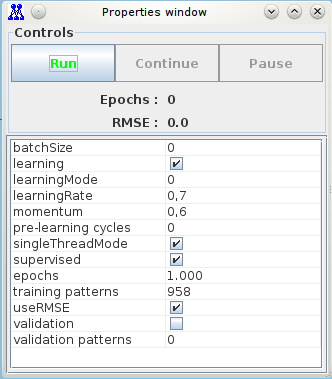
\includegraphics{./Images/configuracion-corridas.png}
 % configuracion-corridas.png: 333x368 pixel, 96dpi, 8.81x9.74 cm, bb=0 0 250 276
\end{center}

Luego del entrenamiento, se obtuvo la siguiente salida; en la cual se puede observar que el error es peque\~no.
\begin{center}
 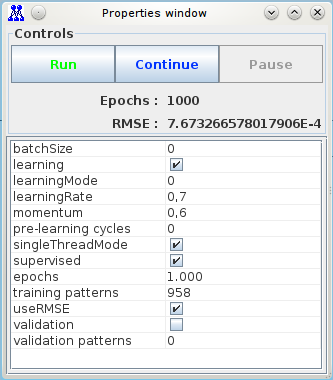
\includegraphics{./Images/fin-corridas.png}
 % fin-corridas.png: 332x366 pixel, 96dpi, 8.78x9.68 cm, bb=0 0 249 274
\end{center}

\section{Resultados}
Luego del aprendizaje que se le aplic\'o a la Red Neuronal, se agreg\'o un archivo de salida para probar la red entrenada. Para ello, se configur\'o: 
\begin{itemize}
 \item learning = FALSE
 \item epochs = 1
\end{itemize}
En el archivo se pudo observar que los valores coinciden apr\'oximadamente con la columna diez de la base de datos original. Se puede observar los resultados en el APENDICE A.

\section{Conclusiones}
En el presente trabajo práctico, nos enfocamos en aprender a utilizar la herramienta Joone y en tener un primer acercamiento a la creaci\'on y entrenamiento de redes neuronales. Como conclusi\'on final podemos decir que el armado de una red neuronal lleva un tiempo considerablemente mayor al del entrenamiento de la misma. Esto se debe a que el entrenamiento es un proceso automatizado, que no requiere m\'as que la configuraci\'on de algunos par\'ametros. Mientras que para el armado de una red neuronal, que nos permita resolver el problema, es necesario un conocimiento sobre la situaci\'on que estamos enfrentando, de manera de poder crear una red que nos permita resolver el problema de manera eficiente. Por otro lado, observamos que el entrenamiento prolongado de una red mal armada no significaba llegar a los resultados deseados. Es decir, que lo m\'as importante es concentrarnos en crear una red acorde al problema; de manera de asegurarnos llegar a los resultados buscados; lo cual puede estar acompa\~nado de un tiempo de entrenamiento m\'as corto de lo esperado. \\

% -------------------------------- Apendice --------------------------------
\appendix
\newpage
\section{Tabla comparativa de los resultados}
A continuaci\'on se presentan los resultados originales de la base de datos contra los obtenidos de la red neuronal entrenada.
\begin{longtable}{|r|r|r|l|r|r|}
\hline
\multicolumn{1}{|l|}{} & \multicolumn{2}{c|}{\textbf{POSITIVOS}} &  & \multicolumn{2}{c|}{\textbf{NEGATIVOS}} \\ \hline
\multicolumn{1}{|l|}{} & \multicolumn{1}{c|}{\textbf{Deseados}} & \multicolumn{1}{c|}{\textbf{Obtenidos}} &  & \multicolumn{1}{c|}{\textbf{Deseados}} & \multicolumn{1}{c|}{\textbf{Obtenidos}} \\ \hline
\textbf{1} & 1 & 0,99890 &  & 0 & 0,00091 \\ \hline
\textbf{2} & 1 & 0,99890 &  & 0 & 0,00090 \\ \hline
\textbf{3} & 1 & 0,99882 &  & 0 & 0,00090 \\ \hline
\textbf{4} & 1 & 0,99890 &  & 0 & 0,00089 \\ \hline
\textbf{5} & 1 & 0,99890 &  & 0 & 0,00090 \\ \hline
\textbf{6} & 1 & 0,99890 &  & 0 & 0,00089 \\ \hline
\textbf{7} & 1 & 0,99890 &  & 0 & 0,00089 \\ \hline
\textbf{8} & 1 & 0,99890 &  & 0 & 0,00089 \\ \hline
\textbf{9} & 1 & 0,99890 &  & 0 & 0,00090 \\ \hline
\textbf{10} & 1 & 0,99890 &  & 0 & 0,00091 \\ \hline
\textbf{11} & 1 & 0,99889 &  & 0 & 0,00089 \\ \hline
\textbf{12} & 1 & 0,99890 &  & 0 & 0,00090 \\ \hline
\textbf{13} & 1 & 0,99890 &  & 0 & 0,00092 \\ \hline
\textbf{14} & 1 & 0,99890 &  & 0 & 0,00096 \\ \hline
\textbf{15} & 1 & 0,99890 &  & 0 & 0,00089 \\ \hline
\textbf{16} & 1 & 0,99890 &  & 0 & 0,00089 \\ \hline
\textbf{17} & 1 & 0,99890 &  & 0 & 0,00090 \\ \hline
\textbf{18} & 1 & 0,99890 &  & 0 & 0,00089 \\ \hline
\textbf{19} & 1 & 0,99889 &  & 0 & 0,00092 \\ \hline
\textbf{20} & 1 & 0,99890 &  & 0 & 0,00089 \\ \hline
\textbf{21} & 1 & 0,99884 &  & 0 & 0,00089 \\ \hline
\textbf{22} & 1 & 0,99889 &  & 0 & 0,00089 \\ \hline
\textbf{23} & 1 & 0,99886 &  & 0 & 0,00099 \\ \hline
\textbf{24} & 1 & 0,99890 &  & 0 & 0,00089 \\ \hline
\textbf{25} & 1 & 0,99890 &  & 0 & 0,00090 \\ \hline
\textbf{26} & 1 & 0,99890 &  & 0 & 0,00090 \\ \hline
\textbf{27} & 1 & 0,99890 &  & 0 & 0,00089 \\ \hline
\textbf{28} & 1 & 0,99889 &  & 0 & 0,00089 \\ \hline
\textbf{29} & 1 & 0,99890 &  & 0 & 0,00089 \\ \hline
\textbf{30} & 1 & 0,99890 &  & 0 & 0,00089 \\ \hline
\textbf{31} & 1 & 0,99890 &  & 0 & 0,00089 \\ \hline
\textbf{32} & 1 & 0,99890 &  & 0 & 0,00089 \\ \hline
\textbf{33} & 1 & 0,99890 &  & 0 & 0,00089 \\ \hline
\textbf{34} & 1 & 0,99890 &  & 0 & 0,00090 \\ \hline
\textbf{35} & 1 & 0,99890 &  & 0 & 0,00090 \\ \hline
\textbf{36} & 1 & 0,99868 &  & 0 & 0,00091 \\ \hline
\textbf{37} & 1 & 0,99885 &  & 0 & 0,00089 \\ \hline
\textbf{38} & 1 & 0,99890 &  & 0 & 0,00093 \\ \hline
\textbf{39} & 1 & 0,99890 &  & 0 & 0,00090 \\ \hline
\textbf{40} & 1 & 0,99890 &  & 0 & 0,00090 \\ \hline
\textbf{41} & 1 & 0,99890 &  & 0 & 0,00091 \\ \hline
\textbf{42} & 1 & 0,99890 &  & 0 & 0,00089 \\ \hline
\textbf{43} & 1 & 0,99890 &  & 0 & 0,00089 \\ \hline
\textbf{44} & 1 & 0,99890 &  & 0 & 0,00090 \\ \hline
\textbf{45} & 1 & 0,99890 &  & 0 & 0,00090 \\ \hline
\textbf{46} & 1 & 0,99890 &  & 0 & 0,00090 \\ \hline
\textbf{47} & 1 & 0,99890 &  & 0 & 0,00093 \\ \hline
\textbf{48} & 1 & 0,99890 &  & 0 & 0,00090 \\ \hline
\textbf{49} & 1 & 0,99890 &  & 0 & 0,00091 \\ \hline
\textbf{50} & 1 & 0,99890 &  & 0 & 0,00089 \\ \hline
\textbf{51} & 1 & 0,99889 &  & 0 & 0,00092 \\ \hline
\textbf{52} & 1 & 0,99890 &  & 0 & 0,00092 \\ \hline
\textbf{53} & 1 & 0,99890 &  & 0 & 0,00101 \\ \hline
\textbf{54} & 1 & 0,99890 &  & 0 & 0,00089 \\ \hline
\textbf{55} & 1 & 0,99890 &  & 0 & 0,00096 \\ \hline
\textbf{56} & 1 & 0,99889 &  & 0 & 0,00091 \\ \hline
\textbf{57} & 1 & 0,99890 &  & 0 & 0,00095 \\ \hline
\textbf{58} & 1 & 0,99890 &  & 0 & 0,00089 \\ \hline
\textbf{59} & 1 & 0,99890 &  & 0 & 0,00099 \\ \hline
\textbf{60} & 1 & 0,99890 &  & 0 & 0,00090 \\ \hline
\textbf{61} & 1 & 0,99890 &  & 0 & 0,00090 \\ \hline
\textbf{62} & 1 & 0,99889 &  & 0 & 0,00089 \\ \hline
\textbf{63} & 1 & 0,99890 &  & 0 & 0,00093 \\ \hline
\textbf{64} & 1 & 0,99890 &  & 0 & 0,00091 \\ \hline
\textbf{65} & 1 & 0,99890 &  & 0 & 0,00090 \\ \hline
\textbf{66} & 1 & 0,99890 &  & 0 & 0,00089 \\ \hline
\textbf{67} & 1 & 0,99890 &  & 0 & 0,00089 \\ \hline
\textbf{68} & 1 & 0,99890 &  & 0 & 0,00092 \\ \hline
\textbf{69} & 1 & 0,99890 &  & 0 & 0,00089 \\ \hline
\textbf{70} & 1 & 0,99890 &  & 0 & 0,00089 \\ \hline
\textbf{71} & 1 & 0,99890 &  & 0 & 0,00090 \\ \hline
\textbf{72} & 1 & 0,99890 &  & 0 & 0,00089 \\ \hline
\textbf{73} & 1 & 0,99890 &  & 0 & 0,00091 \\ \hline
\textbf{74} & 1 & 0,99890 &  & 0 & 0,00092 \\ \hline
\textbf{75} & 1 & 0,99890 &  & 0 & 0,00093 \\ \hline
\textbf{76} & 1 & 0,99890 &  & 0 & 0,00089 \\ \hline
\textbf{77} & 1 & 0,99890 &  & 0 & 0,00089 \\ \hline
\textbf{78} & 1 & 0,99890 &  & 0 & 0,00089 \\ \hline
\textbf{79} & 1 & 0,99890 &  & 0 & 0,00092 \\ \hline
\textbf{80} & 1 & 0,99890 &  & 0 & 0,00093 \\ \hline
\textbf{81} & 1 & 0,99890 &  & 0 & 0,00090 \\ \hline
\textbf{82} & 1 & 0,99889 &  & 0 & 0,00097 \\ \hline
\textbf{83} & 1 & 0,99890 &  & 0 & 0,00093 \\ \hline
\textbf{84} & 1 & 0,99890 &  & 0 & 0,00099 \\ \hline
\textbf{85} & 1 & 0,99890 &  & 0 & 0,00089 \\ \hline
\textbf{86} & 1 & 0,99890 &  & 0 & 0,00091 \\ \hline
\textbf{87} & 1 & 0,99890 &  & 0 & 0,00090 \\ \hline
\textbf{88} & 1 & 0,99890 &  & 0 & 0,00092 \\ \hline
\textbf{89} & 1 & 0,99889 &  & 0 & 0,00091 \\ \hline
\textbf{90} & 1 & 0,99890 &  & 0 & 0,00091 \\ \hline
\textbf{91} & 1 & 0,99890 &  & 0 & 0,00132 \\ \hline
\textbf{92} & 1 & 0,99890 &  & 0 & 0,00090 \\ \hline
\textbf{93} & 1 & 0,99888 &  & 0 & 0,00090 \\ \hline
\textbf{94} & 1 & 0,99890 &  & 0 & 0,00089 \\ \hline
\textbf{95} & 1 & 0,99873 &  & 0 & 0,00090 \\ \hline
\textbf{96} & 1 & 0,99890 &  & 0 & 0,00089 \\ \hline
\textbf{97} & 1 & 0,99890 &  & 0 & 0,00089 \\ \hline
\textbf{98} & 1 & 0,99890 &  & 0 & 0,00089 \\ \hline
\textbf{99} & 1 & 0,99890 &  & 0 & 0,00089 \\ \hline
\textbf{100} & 1 & 0,99890 &  & 0 & 0,00090 \\ \hline
\textbf{101} & 1 & 0,99890 &  & 0 & 0,00089 \\ \hline
\textbf{102} & 1 & 0,99890 &  & 0 & 0,00089 \\ \hline
\textbf{103} & 1 & 0,99890 &  & 0 & 0,00089 \\ \hline
\textbf{104} & 1 & 0,99890 &  & 0 & 0,00090 \\ \hline
\textbf{105} & 1 & 0,99890 &  & 0 & 0,00089 \\ \hline
\textbf{106} & 1 & 0,99890 &  & 0 & 0,00089 \\ \hline
\textbf{107} & 1 & 0,99890 &  & 0 & 0,00089 \\ \hline
\textbf{108} & 1 & 0,99890 &  & 0 & 0,00090 \\ \hline
\textbf{109} & 1 & 0,99890 &  & 0 & 0,00089 \\ \hline
\textbf{110} & 1 & 0,99888 &  & 0 & 0,00093 \\ \hline
\textbf{111} & 1 & 0,99890 &  & 0 & 0,00091 \\ \hline
\textbf{112} & 1 & 0,99890 &  & 0 & 0,00091 \\ \hline
\textbf{113} & 1 & 0,99890 &  & 0 & 0,00091 \\ \hline
\textbf{114} & 1 & 0,99890 &  & 0 & 0,00091 \\ \hline
\textbf{115} & 1 & 0,99890 &  & 0 & 0,00089 \\ \hline
\textbf{116} & 1 & 0,99890 &  & 0 & 0,00140 \\ \hline
\textbf{117} & 1 & 0,99890 &  & 0 & 0,00089 \\ \hline
\textbf{118} & 1 & 0,99890 &  & 0 & 0,00089 \\ \hline
\textbf{119} & 1 & 0,99890 &  & 0 & 0,00090 \\ \hline
\textbf{120} & 1 & 0,99890 &  & 0 & 0,00089 \\ \hline
\textbf{121} & 1 & 0,99890 &  & 0 & 0,00089 \\ \hline
\textbf{122} & 1 & 0,99890 &  & 0 & 0,00089 \\ \hline
\textbf{123} & 1 & 0,99890 &  & 0 & 0,00090 \\ \hline
\textbf{124} & 1 & 0,99888 &  & 0 & 0,00092 \\ \hline
\textbf{125} & 1 & 0,99890 &  & 0 & 0,00091 \\ \hline
\textbf{126} & 1 & 0,99890 &  & 0 & 0,00099 \\ \hline
\textbf{127} & 1 & 0,99889 &  & 0 & 0,00090 \\ \hline
\textbf{128} & 1 & 0,99890 &  & 0 & 0,00093 \\ \hline
\textbf{129} & 1 & 0,99890 &  & 0 & 0,00090 \\ \hline
\textbf{130} & 1 & 0,99890 &  & 0 & 0,00089 \\ \hline
\textbf{131} & 1 & 0,99890 &  & 0 & 0,00089 \\ \hline
\textbf{132} & 1 & 0,99890 &  & 0 & 0,00091 \\ \hline
\textbf{133} & 1 & 0,99890 &  & 0 & 0,00094 \\ \hline
\textbf{134} & 1 & 0,99890 &  & 0 & 0,00091 \\ \hline
\textbf{135} & 1 & 0,99890 &  & 0 & 0,00090 \\ \hline
\textbf{136} & 1 & 0,99890 &  & 0 & 0,00091 \\ \hline
\textbf{137} & 1 & 0,99890 &  & 0 & 0,00091 \\ \hline
\textbf{138} & 1 & 0,99890 &  & 0 & 0,00092 \\ \hline
\textbf{139} & 1 & 0,99890 &  & 0 & 0,00092 \\ \hline
\textbf{140} & 1 & 0,99890 &  & 0 & 0,00096 \\ \hline
\textbf{141} & 1 & 0,99889 &  & 0 & 0,00090 \\ \hline
\textbf{142} & 1 & 0,99890 &  & 0 & 0,00090 \\ \hline
\textbf{143} & 1 & 0,99890 &  & 0 & 0,00090 \\ \hline
\textbf{144} & 1 & 0,99890 &  & 0 & 0,00091 \\ \hline
\textbf{145} & 1 & 0,99890 &  & 0 & 0,00105 \\ \hline
\textbf{146} & 1 & 0,99887 &  & 0 & 0,00091 \\ \hline
\textbf{147} & 1 & 0,99889 &  & 0 & 0,00089 \\ \hline
\textbf{148} & 1 & 0,99890 &  & 0 & 0,00089 \\ \hline
\textbf{149} & 1 & 0,99890 &  & 0 & 0,00089 \\ \hline
\textbf{150} & 1 & 0,99887 &  & 0 & 0,00091 \\ \hline
\textbf{151} & 1 & 0,99890 &  & 0 & 0,00090 \\ \hline
\textbf{152} & 1 & 0,99890 &  & 0 & 0,00094 \\ \hline
\textbf{153} & 1 & 0,99890 &  & 0 & 0,00089 \\ \hline
\textbf{154} & 1 & 0,99890 &  & 0 & 0,00089 \\ \hline
\textbf{155} & 1 & 0,99890 &  & 0 & 0,00092 \\ \hline
\textbf{156} & 1 & 0,99890 &  & 0 & 0,00089 \\ \hline
\textbf{157} & 1 & 0,99890 &  & 0 & 0,00089 \\ \hline
\textbf{158} & 1 & 0,99890 &  & 0 & 0,00091 \\ \hline
\textbf{159} & 1 & 0,99889 &  & 0 & 0,00089 \\ \hline
\textbf{160} & 1 & 0,99709 &  & 0 & 0,00091 \\ \hline
\textbf{161} & 1 & 0,99890 &  & 0 & 0,00095 \\ \hline
\textbf{162} & 1 & 0,99889 &  & 0 & 0,00089 \\ \hline
\textbf{163} & 1 & 0,99890 &  & 0 & 0,00099 \\ \hline
\textbf{164} & 1 & 0,99890 &  & 0 & 0,00093 \\ \hline
\textbf{165} & 1 & 0,99890 &  & 0 & 0,00089 \\ \hline
\textbf{166} & 1 & 0,99890 &  & 0 & 0,00089 \\ \hline
\textbf{167} & 1 & 0,99890 &  & 0 & 0,00093 \\ \hline
\textbf{168} & 1 & 0,99889 &  & 0 & 0,00098 \\ \hline
\textbf{169} & 1 & 0,99890 &  & 0 & 0,00090 \\ \hline
\textbf{170} & 1 & 0,99889 &  & 0 & 0,00089 \\ \hline
\textbf{171} & 1 & 0,99890 &  & 0 & 0,00090 \\ \hline
\textbf{172} & 1 & 0,99889 &  & 0 & 0,00089 \\ \hline
\textbf{173} & 1 & 0,99890 &  & 0 & 0,00089 \\ \hline
\textbf{174} & 1 & 0,99890 &  & 0 & 0,00106 \\ \hline
\textbf{175} & 1 & 0,99890 &  & 0 & 0,00090 \\ \hline
\textbf{176} & 1 & 0,99890 &  & 0 & 0,00089 \\ \hline
\textbf{177} & 1 & 0,99888 &  & 0 & 0,00089 \\ \hline
\textbf{178} & 1 & 0,99890 &  & 0 & 0,00096 \\ \hline
\textbf{179} & 1 & 0,99890 &  & 0 & 0,00100 \\ \hline
\textbf{180} & 1 & 0,99890 &  & 0 & 0,00098 \\ \hline
\textbf{181} & 1 & 0,99890 &  & 0 & 0,00089 \\ \hline
\textbf{182} & 1 & 0,99890 &  & 0 & 0,00096 \\ \hline
\textbf{183} & 1 & 0,99890 &  & 0 & 0,00092 \\ \hline
\textbf{184} & 1 & 0,99890 &  & 0 & 0,00090 \\ \hline
\textbf{185} & 1 & 0,99890 &  & 0 & 0,00090 \\ \hline
\textbf{186} & 1 & 0,99890 &  & 0 & 0,00090 \\ \hline
\textbf{187} & 1 & 0,99890 &  & 0 & 0,00091 \\ \hline
\textbf{188} & 1 & 0,99890 &  & 0 & 0,00113 \\ \hline
\textbf{189} & 1 & 0,99884 &  & 0 & 0,00092 \\ \hline
\textbf{190} & 1 & 0,99890 &  & 0 & 0,00092 \\ \hline
\textbf{191} & 1 & 0,99890 &  & 0 & 0,00090 \\ \hline
\textbf{192} & 1 & 0,99890 &  & 0 & 0,00092 \\ \hline
\textbf{193} & 1 & 0,99890 &  & 0 & 0,00092 \\ \hline
\textbf{194} & 1 & 0,99890 &  & 0 & 0,00089 \\ \hline
\textbf{195} & 1 & 0,99890 &  & 0 & 0,00090 \\ \hline
\textbf{196} & 1 & 0,99890 &  & 0 & 0,00090 \\ \hline
\textbf{197} & 1 & 0,99877 &  & 0 & 0,00097 \\ \hline
\textbf{198} & 1 & 0,99889 &  & 0 & 0,00092 \\ \hline
\textbf{199} & 1 & 0,99890 &  & 0 & 0,00093 \\ \hline
\textbf{200} & 1 & 0,99886 &  & 0 & 0,00098 \\ \hline
\textbf{201} & 1 & 0,99890 &  & 0 & 0,00090 \\ \hline
\textbf{202} & 1 & 0,99890 &  & 0 & 0,00090 \\ \hline
\textbf{203} & 1 & 0,99890 &  & 0 & 0,00090 \\ \hline
\textbf{204} & 1 & 0,99890 &  & 0 & 0,00089 \\ \hline
\textbf{205} & 1 & 0,99890 &  & 0 & 0,00092 \\ \hline
\textbf{206} & 1 & 0,99890 &  & 0 & 0,00090 \\ \hline
\textbf{207} & 1 & 0,99890 &  & 0 & 0,00106 \\ \hline
\textbf{208} & 1 & 0,99890 &  & 0 & 0,00091 \\ \hline
\textbf{209} & 1 & 0,99890 &  & 0 & 0,00090 \\ \hline
\textbf{210} & 1 & 0,99890 &  & 0 & 0,00096 \\ \hline
\textbf{211} & 1 & 0,99890 &  & 0 & 0,00094 \\ \hline
\textbf{212} & 1 & 0,99890 &  & 0 & 0,00090 \\ \hline
\textbf{213} & 1 & 0,99890 &  & 0 & 0,00120 \\ \hline
\textbf{214} & 1 & 0,99890 &  & 0 & 0,00092 \\ \hline
\textbf{215} & 1 & 0,99884 &  & 0 & 0,00090 \\ \hline
\textbf{216} & 1 & 0,99890 &  & 0 & 0,00092 \\ \hline
\textbf{217} & 1 & 0,99890 &  & 0 & 0,00089 \\ \hline
\textbf{218} & 1 & 0,99890 &  & 0 & 0,00089 \\ \hline
\textbf{219} & 1 & 0,99889 &  & 0 & 0,00089 \\ \hline
\textbf{220} & 1 & 0,99890 &  & 0 & 0,00092 \\ \hline
\textbf{221} & 1 & 0,99890 &  & 0 & 0,00089 \\ \hline
\textbf{222} & 1 & 0,99890 &  & 0 & 0,00091 \\ \hline
\textbf{223} & 1 & 0,99884 &  & 0 & 0,00091 \\ \hline
\textbf{224} & 1 & 0,99890 &  & 0 & 0,00091 \\ \hline
\textbf{225} & 1 & 0,99890 &  & 0 & 0,00090 \\ \hline
\textbf{226} & 1 & 0,99890 &  & 0 & 0,00091 \\ \hline
\textbf{227} & 1 & 0,99890 &  & 0 & 0,00089 \\ \hline
\textbf{228} & 1 & 0,99890 &  & 0 & 0,00092 \\ \hline
\textbf{229} & 1 & 0,99890 &  & 0 & 0,00089 \\ \hline
\textbf{230} & 1 & 0,99890 &  & 0 & 0,00089 \\ \hline
\textbf{231} & 1 & 0,99890 &  & 0 & 0,00093 \\ \hline
\textbf{232} & 1 & 0,99889 &  & 0 & 0,00102 \\ \hline
\textbf{233} & 1 & 0,99890 &  & 0 & 0,00094 \\ \hline
\textbf{234} & 1 & 0,99890 &  & 0 & 0,00092 \\ \hline
\textbf{235} & 1 & 0,99890 &  & 0 & 0,00089 \\ \hline
\textbf{236} & 1 & 0,99890 &  & 0 & 0,00089 \\ \hline
\textbf{237} & 1 & 0,99889 &  & 0 & 0,00090 \\ \hline
\textbf{238} & 1 & 0,99890 &  & 0 & 0,00096 \\ \hline
\textbf{239} & 1 & 0,99890 &  & 0 & 0,00090 \\ \hline
\textbf{240} & 1 & 0,99890 &  & 0 & 0,00090 \\ \hline
\textbf{241} & 1 & 0,99882 &  & 0 & 0,00089 \\ \hline
\textbf{242} & 1 & 0,99653 &  & 0 & 0,00089 \\ \hline
\textbf{243} & 1 & 0,99890 &  & 0 & 0,00096 \\ \hline
\textbf{244} & 1 & 0,99890 &  & 0 & 0,00090 \\ \hline
\textbf{245} & 1 & 0,99890 &  & 0 & 0,00091 \\ \hline
\textbf{246} & 1 & 0,99890 &  & 0 & 0,00091 \\ \hline
\textbf{247} & 1 & 0,99890 &  & 0 & 0,00095 \\ \hline
\textbf{248} & 1 & 0,99787 &  & 0 & 0,00089 \\ \hline
\textbf{249} & 1 & 0,99890 &  & 0 & 0,00091 \\ \hline
\textbf{250} & 1 & 0,99889 &  & 0 & 0,00089 \\ \hline
\textbf{251} & 1 & 0,99890 &  & 0 & 0,00095 \\ \hline
\textbf{252} & 1 & 0,99890 &  & 0 & 0,00090 \\ \hline
\textbf{253} & 1 & 0,99889 &  & 0 & 0,00093 \\ \hline
\textbf{254} & 1 & 0,99890 &  & 0 & 0,00115 \\ \hline
\textbf{255} & 1 & 0,99890 &  & 0 & 0,00093 \\ \hline
\textbf{256} & 1 & 0,99890 &  & 0 & 0,00090 \\ \hline
\textbf{257} & 1 & 0,99890 &  & 0 & 0,00090 \\ \hline
\textbf{258} & 1 & 0,99890 &  & 0 & 0,00091 \\ \hline
\textbf{259} & 1 & 0,99890 &  & 0 & 0,00089 \\ \hline
\textbf{260} & 1 & 0,99890 &  & 0 & 0,00091 \\ \hline
\textbf{261} & 1 & 0,99890 &  & 0 & 0,00089 \\ \hline
\textbf{262} & 1 & 0,99889 &  & 0 & 0,00094 \\ \hline
\textbf{263} & 1 & 0,99890 &  & 0 & 0,00128 \\ \hline
\textbf{264} & 1 & 0,99890 &  & 0 & 0,00096 \\ \hline
\textbf{265} & 1 & 0,99890 &  & 0 & 0,00090 \\ \hline
\textbf{266} & 1 & 0,99890 &  & 0 & 0,00089 \\ \hline
\textbf{267} & 1 & 0,99886 &  & 0 & 0,00089 \\ \hline
\textbf{268} & 1 & 0,99888 &  & 0 & 0,00089 \\ \hline
\textbf{269} & 1 & 0,99890 &  & 0 & 0,00089 \\ \hline
\textbf{270} & 1 & 0,99890 &  & 0 & 0,00089 \\ \hline
\textbf{271} & 1 & 0,99890 &  & 0 & 0,00090 \\ \hline
\textbf{272} & 1 & 0,99890 &  & 0 & 0,00089 \\ \hline
\textbf{273} & 1 & 0,99890 &  & 0 & 0,00089 \\ \hline
\textbf{274} & 1 & 0,99890 &  & 0 & 0,00089 \\ \hline
\textbf{275} & 1 & 0,99888 &  & 0 & 0,00089 \\ \hline
\textbf{276} & 1 & 0,99890 &  & 0 & 0,00091 \\ \hline
\textbf{277} & 1 & 0,99890 &  & 0 & 0,00089 \\ \hline
\textbf{278} & 1 & 0,99890 &  & 0 & 0,00090 \\ \hline
\textbf{279} & 1 & 0,99890 &  & 0 & 0,00089 \\ \hline
\textbf{280} & 1 & 0,99890 &  & 0 & 0,00090 \\ \hline
\textbf{281} & 1 & 0,99890 &  & 0 & 0,00089 \\ \hline
\textbf{282} & 1 & 0,99890 &  & 0 & 0,00089 \\ \hline
\textbf{283} & 1 & 0,99890 &  & 0 & 0,00091 \\ \hline
\textbf{284} & 1 & 0,99890 &  & 0 & 0,00089 \\ \hline
\textbf{285} & 1 & 0,99890 &  & 0 & 0,00090 \\ \hline
\textbf{286} & 1 & 0,99889 &  & 0 & 0,00090 \\ \hline
\textbf{287} & 1 & 0,99890 &  & 0 & 0,00089 \\ \hline
\textbf{288} & 1 & 0,99890 &  & 0 & 0,00096 \\ \hline
\textbf{289} & 1 & 0,99889 &  & 0 & 0,00092 \\ \hline
\textbf{290} & 1 & 0,99890 &  & 0 & 0,00095 \\ \hline
\textbf{291} & 1 & 0,99890 &  & 0 & 0,00092 \\ \hline
\textbf{292} & 1 & 0,99890 &  & 0 & 0,00098 \\ \hline
\textbf{293} & 1 & 0,99890 &  & 0 & 0,00118 \\ \hline
\textbf{294} & 1 & 0,99890 &  & 0 & 0,00089 \\ \hline
\textbf{295} & 1 & 0,99890 &  & 0 & 0,00089 \\ \hline
\textbf{296} & 1 & 0,99890 &  & 0 & 0,00089 \\ \hline
\textbf{297} & 1 & 0,99890 &  & 0 & 0,00090 \\ \hline
\textbf{298} & 1 & 0,99890 &  & 0 & 0,00089 \\ \hline
\textbf{299} & 1 & 0,99890 &  & 0 & 0,00091 \\ \hline
\textbf{300} & 1 & 0,99890 &  & 0 & 0,00094 \\ \hline
\textbf{301} & 1 & 0,99890 &  & 0 & 0,00099 \\ \hline
\textbf{302} & 1 & 0,99890 &  & 0 & 0,00089 \\ \hline
\textbf{303} & 1 & 0,99880 &  & 0 & 0,00090 \\ \hline
\textbf{304} & 1 & 0,99890 &  & 0 & 0,00094 \\ \hline
\textbf{305} & 1 & 0,99890 &  & 0 & 0,00092 \\ \hline
\textbf{306} & 1 & 0,99889 &  & 0 & 0,00089 \\ \hline
\textbf{307} & 1 & 0,99885 &  & 0 & 0,00093 \\ \hline
\textbf{308} & 1 & 0,99889 &  & 0 & 0,00092 \\ \hline
\textbf{309} & 1 & 0,99890 &  & 0 & 0,00089 \\ \hline
\textbf{310} & 1 & 0,99890 &  & 0 & 0,00090 \\ \hline
\textbf{311} & 1 & 0,99890 &  & 0 & 0,00089 \\ \hline
\textbf{312} & 1 & 0,99890 &  & 0 & 0,00089 \\ \hline
\textbf{313} & 1 & 0,99890 &  & 0 & 0,00089 \\ \hline
\textbf{314} & 1 & 0,99890 &  & 0 & 0,00090 \\ \hline
\textbf{315} & 1 & 0,99890 &  & 0 & 0,00089 \\ \hline
\textbf{316} & 1 & 0,99890 &  & 0 & 0,00089 \\ \hline
\textbf{317} & 1 & 0,99890 &  & 0 & 0,00322 \\ \hline
\textbf{318} & 1 & 0,99890 &  & 0 & 0,00096 \\ \hline
\textbf{319} & 1 & 0,99890 &  & 0 & 0,00090 \\ \hline
\textbf{320} & 1 & 0,99890 &  & 0 & 0,00170 \\ \hline
\textbf{321} & 1 & 0,99888 &  & 0 & 0,00299 \\ \hline
\textbf{322} & 1 & 0,99890 &  & 0 & 0,00119 \\ \hline
\textbf{323} & 1 & 0,99885 &  & 0 & 0,00208 \\ \hline
\textbf{324} & 1 & 0,99890 &  & 0 & 0,00230 \\ \hline
\textbf{325} & 1 & 0,99890 &  & 0 & 0,00091 \\ \hline
\textbf{326} & 1 & 0,99890 &  & 0 & 0,00247 \\ \hline
\textbf{327} & 1 & 0,99890 &  & 0 & 0,00151 \\ \hline
\textbf{328} & 1 & 0,99890 &  & 0 & 0,00117 \\ \hline
\textbf{329} & 1 & 0,99890 &  & 0 & 0,00098 \\ \hline
\textbf{330} & 1 & 0,99885 &  & 0 & 0,00146 \\ \hline
\textbf{331} & 1 & 0,99782 &  & 0 & 0,00103 \\ \hline
\textbf{332} & 1 & 0,99890 &  & 0 & 0,00153 \\ \hline
\textbf{333} & 1 & 0,99889 &  & \multicolumn{1}{l|}{} & \multicolumn{1}{l|}{} \\ \hline
\textbf{334} & 1 & 0,99890 &  & \multicolumn{1}{l|}{} & \multicolumn{1}{l|}{} \\ \hline
\textbf{335} & 1 & 0,99879 &  & \multicolumn{1}{l|}{} & \multicolumn{1}{l|}{} \\ \hline
\textbf{336} & 1 & 0,99889 &  & \multicolumn{1}{l|}{} & \multicolumn{1}{l|}{} \\ \hline
\textbf{337} & 1 & 0,99890 &  & \multicolumn{1}{l|}{} & \multicolumn{1}{l|}{} \\ \hline
\textbf{338} & 1 & 0,99890 &  & \multicolumn{1}{l|}{} & \multicolumn{1}{l|}{} \\ \hline
\textbf{339} & 1 & 0,99890 &  & \multicolumn{1}{l|}{} & \multicolumn{1}{l|}{} \\ \hline
\textbf{340} & 1 & 0,99890 &  & \multicolumn{1}{l|}{} & \multicolumn{1}{l|}{} \\ \hline
\textbf{341} & 1 & 0,99835 &  & \multicolumn{1}{l|}{} & \multicolumn{1}{l|}{} \\ \hline
\textbf{342} & 1 & 0,99890 &  & \multicolumn{1}{l|}{} & \multicolumn{1}{l|}{} \\ \hline
\textbf{343} & 1 & 0,99889 &  & \multicolumn{1}{l|}{} & \multicolumn{1}{l|}{} \\ \hline
\textbf{344} & 1 & 0,99890 &  & \multicolumn{1}{l|}{} & \multicolumn{1}{l|}{} \\ \hline
\textbf{345} & 1 & 0,99880 &  & \multicolumn{1}{l|}{} & \multicolumn{1}{l|}{} \\ \hline
\textbf{346} & 1 & 0,99887 &  & \multicolumn{1}{l|}{} & \multicolumn{1}{l|}{} \\ \hline
\textbf{347} & 1 & 0,99890 &  & \multicolumn{1}{l|}{} & \multicolumn{1}{l|}{} \\ \hline
\textbf{348} & 1 & 0,99890 &  & \multicolumn{1}{l|}{} & \multicolumn{1}{l|}{} \\ \hline
\textbf{349} & 1 & 0,99890 &  & \multicolumn{1}{l|}{} & \multicolumn{1}{l|}{} \\ \hline
\textbf{350} & 1 & 0,99890 &  & \multicolumn{1}{l|}{} & \multicolumn{1}{l|}{} \\ \hline
\textbf{351} & 1 & 0,99890 &  & \multicolumn{1}{l|}{} & \multicolumn{1}{l|}{} \\ \hline
\textbf{352} & 1 & 0,99890 &  & \multicolumn{1}{l|}{} & \multicolumn{1}{l|}{} \\ \hline
\textbf{353} & 1 & 0,99889 &  & \multicolumn{1}{l|}{} & \multicolumn{1}{l|}{} \\ \hline
\textbf{354} & 1 & 0,99886 &  & \multicolumn{1}{l|}{} & \multicolumn{1}{l|}{} \\ \hline
\textbf{355} & 1 & 0,99855 &  & \multicolumn{1}{l|}{} & \multicolumn{1}{l|}{} \\ \hline
\textbf{356} & 1 & 0,99890 &  & \multicolumn{1}{l|}{} & \multicolumn{1}{l|}{} \\ \hline
\textbf{357} & 1 & 0,99890 &  & \multicolumn{1}{l|}{} & \multicolumn{1}{l|}{} \\ \hline
\textbf{358} & 1 & 0,99888 &  & \multicolumn{1}{l|}{} & \multicolumn{1}{l|}{} \\ \hline
\textbf{359} & 1 & 0,99890 &  & \multicolumn{1}{l|}{} & \multicolumn{1}{l|}{} \\ \hline
\textbf{360} & 1 & 0,99889 &  & \multicolumn{1}{l|}{} & \multicolumn{1}{l|}{} \\ \hline
\textbf{361} & 1 & 0,99885 &  & \multicolumn{1}{l|}{} & \multicolumn{1}{l|}{} \\ \hline
\textbf{362} & 1 & 0,99890 &  & \multicolumn{1}{l|}{} & \multicolumn{1}{l|}{} \\ \hline
\textbf{363} & 1 & 0,99890 &  & \multicolumn{1}{l|}{} & \multicolumn{1}{l|}{} \\ \hline
\textbf{364} & 1 & 0,99889 &  & \multicolumn{1}{l|}{} & \multicolumn{1}{l|}{} \\ \hline
\textbf{365} & 1 & 0,99890 &  & \multicolumn{1}{l|}{} & \multicolumn{1}{l|}{} \\ \hline
\textbf{366} & 1 & 0,99890 &  & \multicolumn{1}{l|}{} & \multicolumn{1}{l|}{} \\ \hline
\textbf{367} & 1 & 0,99890 &  & \multicolumn{1}{l|}{} & \multicolumn{1}{l|}{} \\ \hline
\textbf{368} & 1 & 0,99890 &  & \multicolumn{1}{l|}{} & \multicolumn{1}{l|}{} \\ \hline
\textbf{369} & 1 & 0,99890 &  & \multicolumn{1}{l|}{} & \multicolumn{1}{l|}{} \\ \hline
\textbf{370} & 1 & 0,99890 &  & \multicolumn{1}{l|}{} & \multicolumn{1}{l|}{} \\ \hline
\textbf{371} & 1 & 0,99890 &  & \multicolumn{1}{l|}{} & \multicolumn{1}{l|}{} \\ \hline
\textbf{372} & 1 & 0,99888 &  & \multicolumn{1}{l|}{} & \multicolumn{1}{l|}{} \\ \hline
\textbf{373} & 1 & 0,99850 &  & \multicolumn{1}{l|}{} & \multicolumn{1}{l|}{} \\ \hline
\textbf{374} & 1 & 0,99884 &  & \multicolumn{1}{l|}{} & \multicolumn{1}{l|}{} \\ \hline
\textbf{375} & 1 & 0,99890 &  & \multicolumn{1}{l|}{} & \multicolumn{1}{l|}{} \\ \hline
\textbf{376} & 1 & 0,99890 &  & \multicolumn{1}{l|}{} & \multicolumn{1}{l|}{} \\ \hline
\textbf{377} & 1 & 0,99890 &  & \multicolumn{1}{l|}{} & \multicolumn{1}{l|}{} \\ \hline
\textbf{378} & 1 & 0,99889 &  & \multicolumn{1}{l|}{} & \multicolumn{1}{l|}{} \\ \hline
\textbf{379} & 1 & 0,99890 &  & \multicolumn{1}{l|}{} & \multicolumn{1}{l|}{} \\ \hline
\textbf{380} & 1 & 0,99890 &  & \multicolumn{1}{l|}{} & \multicolumn{1}{l|}{} \\ \hline
\textbf{381} & 1 & 0,99890 &  & \multicolumn{1}{l|}{} & \multicolumn{1}{l|}{} \\ \hline
\textbf{382} & 1 & 0,99890 &  & \multicolumn{1}{l|}{} & \multicolumn{1}{l|}{} \\ \hline
\textbf{383} & 1 & 0,99890 &  & \multicolumn{1}{l|}{} & \multicolumn{1}{l|}{} \\ \hline
\textbf{384} & 1 & 0,99890 &  & \multicolumn{1}{l|}{} & \multicolumn{1}{l|}{} \\ \hline
\textbf{385} & 1 & 0,99890 &  & \multicolumn{1}{l|}{} & \multicolumn{1}{l|}{} \\ \hline
\textbf{386} & 1 & 0,99890 &  & \multicolumn{1}{l|}{} & \multicolumn{1}{l|}{} \\ \hline
\textbf{387} & 1 & 0,99890 &  & \multicolumn{1}{l|}{} & \multicolumn{1}{l|}{} \\ \hline
\textbf{388} & 1 & 0,99890 &  & \multicolumn{1}{l|}{} & \multicolumn{1}{l|}{} \\ \hline
\textbf{389} & 1 & 0,99890 &  & \multicolumn{1}{l|}{} & \multicolumn{1}{l|}{} \\ \hline
\textbf{390} & 1 & 0,99889 &  & \multicolumn{1}{l|}{} & \multicolumn{1}{l|}{} \\ \hline
\textbf{391} & 1 & 0,99890 &  & \multicolumn{1}{l|}{} & \multicolumn{1}{l|}{} \\ \hline
\textbf{392} & 1 & 0,99890 &  & \multicolumn{1}{l|}{} & \multicolumn{1}{l|}{} \\ \hline
\textbf{393} & 1 & 0,99890 &  & \multicolumn{1}{l|}{} & \multicolumn{1}{l|}{} \\ \hline
\textbf{394} & 1 & 0,99890 &  & \multicolumn{1}{l|}{} & \multicolumn{1}{l|}{} \\ \hline
\textbf{395} & 1 & 0,99890 &  & \multicolumn{1}{l|}{} & \multicolumn{1}{l|}{} \\ \hline
\textbf{396} & 1 & 0,99890 &  & \multicolumn{1}{l|}{} & \multicolumn{1}{l|}{} \\ \hline
\textbf{397} & 1 & 0,99890 &  & \multicolumn{1}{l|}{} & \multicolumn{1}{l|}{} \\ \hline
\textbf{398} & 1 & 0,99889 &  & \multicolumn{1}{l|}{} & \multicolumn{1}{l|}{} \\ \hline
\textbf{399} & 1 & 0,99890 &  & \multicolumn{1}{l|}{} & \multicolumn{1}{l|}{} \\ \hline
\textbf{400} & 1 & 0,99890 &  & \multicolumn{1}{l|}{} & \multicolumn{1}{l|}{} \\ \hline
\textbf{401} & 1 & 0,99890 &  & \multicolumn{1}{l|}{} & \multicolumn{1}{l|}{} \\ \hline
\textbf{402} & 1 & 0,99846 &  & \multicolumn{1}{l|}{} & \multicolumn{1}{l|}{} \\ \hline
\textbf{403} & 1 & 0,99890 &  & \multicolumn{1}{l|}{} & \multicolumn{1}{l|}{} \\ \hline
\textbf{404} & 1 & 0,99890 &  & \multicolumn{1}{l|}{} & \multicolumn{1}{l|}{} \\ \hline
\textbf{405} & 1 & 0,99890 &  & \multicolumn{1}{l|}{} & \multicolumn{1}{l|}{} \\ \hline
\textbf{406} & 1 & 0,99889 &  & \multicolumn{1}{l|}{} & \multicolumn{1}{l|}{} \\ \hline
\textbf{407} & 1 & 0,99890 &  & \multicolumn{1}{l|}{} & \multicolumn{1}{l|}{} \\ \hline
\textbf{408} & 1 & 0,99890 &  & \multicolumn{1}{l|}{} & \multicolumn{1}{l|}{} \\ \hline
\textbf{409} & 1 & 0,99886 &  & \multicolumn{1}{l|}{} & \multicolumn{1}{l|}{} \\ \hline
\textbf{410} & 1 & 0,99890 &  & \multicolumn{1}{l|}{} & \multicolumn{1}{l|}{} \\ \hline
\textbf{411} & 1 & 0,99889 &  & \multicolumn{1}{l|}{} & \multicolumn{1}{l|}{} \\ \hline
\textbf{412} & 1 & 0,99889 &  & \multicolumn{1}{l|}{} & \multicolumn{1}{l|}{} \\ \hline
\textbf{413} & 1 & 0,99890 &  & \multicolumn{1}{l|}{} & \multicolumn{1}{l|}{} \\ \hline
\textbf{414} & 1 & 0,99890 &  & \multicolumn{1}{l|}{} & \multicolumn{1}{l|}{} \\ \hline
\textbf{415} & 1 & 0,99889 &  & \multicolumn{1}{l|}{} & \multicolumn{1}{l|}{} \\ \hline
\textbf{416} & 1 & 0,99890 &  & \multicolumn{1}{l|}{} & \multicolumn{1}{l|}{} \\ \hline
\textbf{417} & 1 & 0,99890 &  & \multicolumn{1}{l|}{} & \multicolumn{1}{l|}{} \\ \hline
\textbf{418} & 1 & 0,99889 &  & \multicolumn{1}{l|}{} & \multicolumn{1}{l|}{} \\ \hline
\textbf{419} & 1 & 0,99890 &  & \multicolumn{1}{l|}{} & \multicolumn{1}{l|}{} \\ \hline
\textbf{420} & 1 & 0,99885 &  & \multicolumn{1}{l|}{} & \multicolumn{1}{l|}{} \\ \hline
\textbf{421} & 1 & 0,99837 &  & \multicolumn{1}{l|}{} & \multicolumn{1}{l|}{} \\ \hline
\textbf{422} & 1 & 0,99890 &  & \multicolumn{1}{l|}{} & \multicolumn{1}{l|}{} \\ \hline
\textbf{423} & 1 & 0,99889 &  & \multicolumn{1}{l|}{} & \multicolumn{1}{l|}{} \\ \hline
\textbf{424} & 1 & 0,99888 &  & \multicolumn{1}{l|}{} & \multicolumn{1}{l|}{} \\ \hline
\textbf{425} & 1 & 0,99890 &  & \multicolumn{1}{l|}{} & \multicolumn{1}{l|}{} \\ \hline
\textbf{426} & 1 & 0,99890 &  & \multicolumn{1}{l|}{} & \multicolumn{1}{l|}{} \\ \hline
\textbf{427} & 1 & 0,99890 &  & \multicolumn{1}{l|}{} & \multicolumn{1}{l|}{} \\ \hline
\textbf{428} & 1 & 0,99890 &  & \multicolumn{1}{l|}{} & \multicolumn{1}{l|}{} \\ \hline
\textbf{429} & 1 & 0,99890 &  & \multicolumn{1}{l|}{} & \multicolumn{1}{l|}{} \\ \hline
\textbf{430} & 1 & 0,99890 &  & \multicolumn{1}{l|}{} & \multicolumn{1}{l|}{} \\ \hline
\textbf{431} & 1 & 0,99890 &  & \multicolumn{1}{l|}{} & \multicolumn{1}{l|}{} \\ \hline
\textbf{432} & 1 & 0,99890 &  & \multicolumn{1}{l|}{} & \multicolumn{1}{l|}{} \\ \hline
\textbf{433} & 1 & 0,99890 &  & \multicolumn{1}{l|}{} & \multicolumn{1}{l|}{} \\ \hline
\textbf{434} & 1 & 0,99890 &  & \multicolumn{1}{l|}{} & \multicolumn{1}{l|}{} \\ \hline
\textbf{435} & 1 & 0,99890 &  & \multicolumn{1}{l|}{} & \multicolumn{1}{l|}{} \\ \hline
\textbf{436} & 1 & 0,99890 &  & \multicolumn{1}{l|}{} & \multicolumn{1}{l|}{} \\ \hline
\textbf{437} & 1 & 0,99890 &  & \multicolumn{1}{l|}{} & \multicolumn{1}{l|}{} \\ \hline
\textbf{438} & 1 & 0,99890 &  & \multicolumn{1}{l|}{} & \multicolumn{1}{l|}{} \\ \hline
\textbf{439} & 1 & 0,99890 &  & \multicolumn{1}{l|}{} & \multicolumn{1}{l|}{} \\ \hline
\textbf{440} & 1 & 0,99890 &  & \multicolumn{1}{l|}{} & \multicolumn{1}{l|}{} \\ \hline
\textbf{441} & 1 & 0,99890 &  & \multicolumn{1}{l|}{} & \multicolumn{1}{l|}{} \\ \hline
\textbf{442} & 1 & 0,99890 &  & \multicolumn{1}{l|}{} & \multicolumn{1}{l|}{} \\ \hline
\textbf{443} & 1 & 0,99889 &  & \multicolumn{1}{l|}{} & \multicolumn{1}{l|}{} \\ \hline
\textbf{444} & 1 & 0,99890 &  & \multicolumn{1}{l|}{} & \multicolumn{1}{l|}{} \\ \hline
\textbf{445} & 1 & 0,99890 &  & \multicolumn{1}{l|}{} & \multicolumn{1}{l|}{} \\ \hline
\textbf{446} & 1 & 0,99890 &  & \multicolumn{1}{l|}{} & \multicolumn{1}{l|}{} \\ \hline
\textbf{447} & 1 & 0,99890 &  & \multicolumn{1}{l|}{} & \multicolumn{1}{l|}{} \\ \hline
\textbf{448} & 1 & 0,99890 &  & \multicolumn{1}{l|}{} & \multicolumn{1}{l|}{} \\ \hline
\textbf{449} & 1 & 0,99889 &  & \multicolumn{1}{l|}{} & \multicolumn{1}{l|}{} \\ \hline
\textbf{450} & 1 & 0,99890 &  & \multicolumn{1}{l|}{} & \multicolumn{1}{l|}{} \\ \hline
\textbf{451} & 1 & 0,99890 &  & \multicolumn{1}{l|}{} & \multicolumn{1}{l|}{} \\ \hline
\textbf{452} & 1 & 0,99890 &  & \multicolumn{1}{l|}{} & \multicolumn{1}{l|}{} \\ \hline
\textbf{453} & 1 & 0,99890 &  & \multicolumn{1}{l|}{} & \multicolumn{1}{l|}{} \\ \hline
\textbf{454} & 1 & 0,99890 &  & \multicolumn{1}{l|}{} & \multicolumn{1}{l|}{} \\ \hline
\textbf{455} & 1 & 0,99890 &  & \multicolumn{1}{l|}{} & \multicolumn{1}{l|}{} \\ \hline
\textbf{456} & 1 & 0,99869 &  & \multicolumn{1}{l|}{} & \multicolumn{1}{l|}{} \\ \hline
\textbf{457} & 1 & 0,99890 &  & \multicolumn{1}{l|}{} & \multicolumn{1}{l|}{} \\ \hline
\textbf{458} & 1 & 0,99890 &  & \multicolumn{1}{l|}{} & \multicolumn{1}{l|}{} \\ \hline
\textbf{459} & 1 & 0,99884 &  & \multicolumn{1}{l|}{} & \multicolumn{1}{l|}{} \\ \hline
\textbf{460} & 1 & 0,99884 &  & \multicolumn{1}{l|}{} & \multicolumn{1}{l|}{} \\ \hline
\textbf{461} & 1 & 0,99887 &  & \multicolumn{1}{l|}{} & \multicolumn{1}{l|}{} \\ \hline
\textbf{462} & 1 & 0,99876 &  & \multicolumn{1}{l|}{} & \multicolumn{1}{l|}{} \\ \hline
\textbf{463} & 1 & 0,99889 &  & \multicolumn{1}{l|}{} & \multicolumn{1}{l|}{} \\ \hline
\textbf{464} & 1 & 0,99882 &  & \multicolumn{1}{l|}{} & \multicolumn{1}{l|}{} \\ \hline
\textbf{465} & 1 & 0,99818 &  & \multicolumn{1}{l|}{} & \multicolumn{1}{l|}{} \\ \hline
\textbf{466} & 1 & 0,99890 &  & \multicolumn{1}{l|}{} & \multicolumn{1}{l|}{} \\ \hline
\textbf{467} & 1 & 0,99881 &  & \multicolumn{1}{l|}{} & \multicolumn{1}{l|}{} \\ \hline
\textbf{468} & 1 & 0,99890 &  & \multicolumn{1}{l|}{} & \multicolumn{1}{l|}{} \\ \hline
\textbf{469} & 1 & 0,99865 &  & \multicolumn{1}{l|}{} & \multicolumn{1}{l|}{} \\ \hline
\textbf{470} & 1 & 0,99890 &  & \multicolumn{1}{l|}{} & \multicolumn{1}{l|}{} \\ \hline
\textbf{471} & 1 & 0,99877 &  & \multicolumn{1}{l|}{} & \multicolumn{1}{l|}{} \\ \hline
\textbf{472} & 1 & 0,99884 &  & \multicolumn{1}{l|}{} & \multicolumn{1}{l|}{} \\ \hline
\textbf{473} & 1 & 0,99890 &  & \multicolumn{1}{l|}{} & \multicolumn{1}{l|}{} \\ \hline
\textbf{474} & 1 & 0,99890 &  & \multicolumn{1}{l|}{} & \multicolumn{1}{l|}{} \\ \hline
\textbf{475} & 1 & 0,99890 &  & \multicolumn{1}{l|}{} & \multicolumn{1}{l|}{} \\ \hline
\textbf{476} & 1 & 0,99890 &  & \multicolumn{1}{l|}{} & \multicolumn{1}{l|}{} \\ \hline
\textbf{477} & 1 & 0,99889 &  & \multicolumn{1}{l|}{} & \multicolumn{1}{l|}{} \\ \hline
\textbf{478} & 1 & 0,99890 &  & \multicolumn{1}{l|}{} & \multicolumn{1}{l|}{} \\ \hline
\textbf{479} & 1 & 0,99890 &  & \multicolumn{1}{l|}{} & \multicolumn{1}{l|}{} \\ \hline
\textbf{480} & 1 & 0,99890 &  & \multicolumn{1}{l|}{} & \multicolumn{1}{l|}{} \\ \hline
\textbf{481} & 1 & 0,99890 &  & \multicolumn{1}{l|}{} & \multicolumn{1}{l|}{} \\ \hline
\textbf{482} & 1 & 0,99890 &  & \multicolumn{1}{l|}{} & \multicolumn{1}{l|}{} \\ \hline
\textbf{483} & 1 & 0,99890 &  & \multicolumn{1}{l|}{} & \multicolumn{1}{l|}{} \\ \hline
\textbf{484} & 1 & 0,99890 &  & \multicolumn{1}{l|}{} & \multicolumn{1}{l|}{} \\ \hline
\textbf{485} & 1 & 0,99890 &  & \multicolumn{1}{l|}{} & \multicolumn{1}{l|}{} \\ \hline
\textbf{486} & 1 & 0,99890 &  & \multicolumn{1}{l|}{} & \multicolumn{1}{l|}{} \\ \hline
\textbf{487} & 1 & 0,99890 &  & \multicolumn{1}{l|}{} & \multicolumn{1}{l|}{} \\ \hline
\textbf{488} & 1 & 0,99890 &  & \multicolumn{1}{l|}{} & \multicolumn{1}{l|}{} \\ \hline
\textbf{489} & 1 & 0,99890 &  & \multicolumn{1}{l|}{} & \multicolumn{1}{l|}{} \\ \hline
\textbf{490} & 1 & 0,99890 &  & \multicolumn{1}{l|}{} & \multicolumn{1}{l|}{} \\ \hline
\textbf{491} & 1 & 0,99890 &  & \multicolumn{1}{l|}{} & \multicolumn{1}{l|}{} \\ \hline
\textbf{492} & 1 & 0,99890 &  & \multicolumn{1}{l|}{} & \multicolumn{1}{l|}{} \\ \hline
\textbf{493} & 1 & 0,99890 &  & \multicolumn{1}{l|}{} & \multicolumn{1}{l|}{} \\ \hline
\textbf{494} & 1 & 0,99890 &  & \multicolumn{1}{l|}{} & \multicolumn{1}{l|}{} \\ \hline
\textbf{495} & 1 & 0,99890 &  & \multicolumn{1}{l|}{} & \multicolumn{1}{l|}{} \\ \hline
\textbf{496} & 1 & 0,99890 &  & \multicolumn{1}{l|}{} & \multicolumn{1}{l|}{} \\ \hline
\textbf{497} & 1 & 0,99890 &  & \multicolumn{1}{l|}{} & \multicolumn{1}{l|}{} \\ \hline
\textbf{498} & 1 & 0,99890 &  & \multicolumn{1}{l|}{} & \multicolumn{1}{l|}{} \\ \hline
\textbf{499} & 1 & 0,99888 &  & \multicolumn{1}{l|}{} & \multicolumn{1}{l|}{} \\ \hline
\textbf{500} & 1 & 0,99890 &  & \multicolumn{1}{l|}{} & \multicolumn{1}{l|}{} \\ \hline
\textbf{501} & 1 & 0,99890 &  & \multicolumn{1}{l|}{} & \multicolumn{1}{l|}{} \\ \hline
\textbf{502} & 1 & 0,99890 &  & \multicolumn{1}{l|}{} & \multicolumn{1}{l|}{} \\ \hline
\textbf{503} & 1 & 0,99890 &  & \multicolumn{1}{l|}{} & \multicolumn{1}{l|}{} \\ \hline
\textbf{504} & 1 & 0,99889 &  & \multicolumn{1}{l|}{} & \multicolumn{1}{l|}{} \\ \hline
\textbf{505} & 1 & 0,99890 &  & \multicolumn{1}{l|}{} & \multicolumn{1}{l|}{} \\ \hline
\textbf{506} & 1 & 0,99887 &  & \multicolumn{1}{l|}{} & \multicolumn{1}{l|}{} \\ \hline
\textbf{507} & 1 & 0,99890 &  & \multicolumn{1}{l|}{} & \multicolumn{1}{l|}{} \\ \hline
\textbf{508} & 1 & 0,99890 &  & \multicolumn{1}{l|}{} & \multicolumn{1}{l|}{} \\ \hline
\textbf{509} & 1 & 0,99888 &  & \multicolumn{1}{l|}{} & \multicolumn{1}{l|}{} \\ \hline
\textbf{510} & 1 & 0,99889 &  & \multicolumn{1}{l|}{} & \multicolumn{1}{l|}{} \\ \hline
\textbf{511} & 1 & 0,99890 &  & \multicolumn{1}{l|}{} & \multicolumn{1}{l|}{} \\ \hline
\textbf{512} & 1 & 0,99890 &  & \multicolumn{1}{l|}{} & \multicolumn{1}{l|}{} \\ \hline
\textbf{513} & 1 & 0,99890 &  & \multicolumn{1}{l|}{} & \multicolumn{1}{l|}{} \\ \hline
\textbf{514} & 1 & 0,99890 &  & \multicolumn{1}{l|}{} & \multicolumn{1}{l|}{} \\ \hline
\textbf{515} & 1 & 0,99890 &  & \multicolumn{1}{l|}{} & \multicolumn{1}{l|}{} \\ \hline
\textbf{516} & 1 & 0,99890 &  & \multicolumn{1}{l|}{} & \multicolumn{1}{l|}{} \\ \hline
\textbf{517} & 1 & 0,99890 &  & \multicolumn{1}{l|}{} & \multicolumn{1}{l|}{} \\ \hline
\textbf{518} & 1 & 0,99886 &  & \multicolumn{1}{l|}{} & \multicolumn{1}{l|}{} \\ \hline
\textbf{519} & 1 & 0,99888 &  & \multicolumn{1}{l|}{} & \multicolumn{1}{l|}{} \\ \hline
\textbf{520} & 1 & 0,99888 &  & \multicolumn{1}{l|}{} & \multicolumn{1}{l|}{} \\ \hline
\textbf{521} & 1 & 0,99890 &  & \multicolumn{1}{l|}{} & \multicolumn{1}{l|}{} \\ \hline
\textbf{522} & 1 & 0,99890 &  & \multicolumn{1}{l|}{} & \multicolumn{1}{l|}{} \\ \hline
\textbf{523} & 1 & 0,99887 &  & \multicolumn{1}{l|}{} & \multicolumn{1}{l|}{} \\ \hline
\textbf{524} & 1 & 0,99890 &  & \multicolumn{1}{l|}{} & \multicolumn{1}{l|}{} \\ \hline
\textbf{525} & 1 & 0,99890 &  & \multicolumn{1}{l|}{} & \multicolumn{1}{l|}{} \\ \hline
\textbf{526} & 1 & 0,99890 &  & \multicolumn{1}{l|}{} & \multicolumn{1}{l|}{} \\ \hline
\textbf{527} & 1 & 0,99890 &  & \multicolumn{1}{l|}{} & \multicolumn{1}{l|}{} \\ \hline
\textbf{528} & 1 & 0,99890 &  & \multicolumn{1}{l|}{} & \multicolumn{1}{l|}{} \\ \hline
\textbf{529} & 1 & 0,99890 &  & \multicolumn{1}{l|}{} & \multicolumn{1}{l|}{} \\ \hline
\textbf{530} & 1 & 0,99890 &  & \multicolumn{1}{l|}{} & \multicolumn{1}{l|}{} \\ \hline
\textbf{531} & 1 & 0,99890 &  & \multicolumn{1}{l|}{} & \multicolumn{1}{l|}{} \\ \hline
\textbf{532} & 1 & 0,99890 &  & \multicolumn{1}{l|}{} & \multicolumn{1}{l|}{} \\ \hline
\textbf{533} & 1 & 0,99887 &  & \multicolumn{1}{l|}{} & \multicolumn{1}{l|}{} \\ \hline
\textbf{534} & 1 & 0,99890 &  & \multicolumn{1}{l|}{} & \multicolumn{1}{l|}{} \\ \hline
\textbf{535} & 1 & 0,99890 &  & \multicolumn{1}{l|}{} & \multicolumn{1}{l|}{} \\ \hline
\textbf{536} & 1 & 0,99890 &  & \multicolumn{1}{l|}{} & \multicolumn{1}{l|}{} \\ \hline
\textbf{537} & 1 & 0,99890 &  & \multicolumn{1}{l|}{} & \multicolumn{1}{l|}{} \\ \hline
\textbf{538} & 1 & 0,99890 &  & \multicolumn{1}{l|}{} & \multicolumn{1}{l|}{} \\ \hline
\textbf{539} & 1 & 0,99890 &  & \multicolumn{1}{l|}{} & \multicolumn{1}{l|}{} \\ \hline
\textbf{540} & 1 & 0,99890 &  & \multicolumn{1}{l|}{} & \multicolumn{1}{l|}{} \\ \hline
\textbf{541} & 1 & 0,99890 &  & \multicolumn{1}{l|}{} & \multicolumn{1}{l|}{} \\ \hline
\textbf{542} & 1 & 0,99890 &  & \multicolumn{1}{l|}{} & \multicolumn{1}{l|}{} \\ \hline
\textbf{543} & 1 & 0,99890 &  & \multicolumn{1}{l|}{} & \multicolumn{1}{l|}{} \\ \hline
\textbf{544} & 1 & 0,99886 &  & \multicolumn{1}{l|}{} & \multicolumn{1}{l|}{} \\ \hline
\textbf{545} & 1 & 0,99890 &  & \multicolumn{1}{l|}{} & \multicolumn{1}{l|}{} \\ \hline
\textbf{546} & 1 & 0,99883 &  & \multicolumn{1}{l|}{} & \multicolumn{1}{l|}{} \\ \hline
\textbf{547} & 1 & 0,99890 &  & \multicolumn{1}{l|}{} & \multicolumn{1}{l|}{} \\ \hline
\textbf{548} & 1 & 0,99890 &  & \multicolumn{1}{l|}{} & \multicolumn{1}{l|}{} \\ \hline
\textbf{549} & 1 & 0,99890 &  & \multicolumn{1}{l|}{} & \multicolumn{1}{l|}{} \\ \hline
\textbf{550} & 1 & 0,99890 &  & \multicolumn{1}{l|}{} & \multicolumn{1}{l|}{} \\ \hline
\textbf{551} & 1 & 0,99890 &  & \multicolumn{1}{l|}{} & \multicolumn{1}{l|}{} \\ \hline
\textbf{552} & 1 & 0,99890 &  & \multicolumn{1}{l|}{} & \multicolumn{1}{l|}{} \\ \hline
\textbf{553} & 1 & 0,99888 &  & \multicolumn{1}{l|}{} & \multicolumn{1}{l|}{} \\ \hline
\textbf{554} & 1 & 0,99890 &  & \multicolumn{1}{l|}{} & \multicolumn{1}{l|}{} \\ \hline
\textbf{555} & 1 & 0,99890 &  & \multicolumn{1}{l|}{} & \multicolumn{1}{l|}{} \\ \hline
\textbf{556} & 1 & 0,99890 &  & \multicolumn{1}{l|}{} & \multicolumn{1}{l|}{} \\ \hline
\textbf{557} & 1 & 0,99890 &  & \multicolumn{1}{l|}{} & \multicolumn{1}{l|}{} \\ \hline
\textbf{558} & 1 & 0,99890 &  & \multicolumn{1}{l|}{} & \multicolumn{1}{l|}{} \\ \hline
\textbf{559} & 1 & 0,99889 &  & \multicolumn{1}{l|}{} & \multicolumn{1}{l|}{} \\ \hline
\textbf{560} & 1 & 0,99870 &  & \multicolumn{1}{l|}{} & \multicolumn{1}{l|}{} \\ \hline
\textbf{561} & 1 & 0,99890 &  & \multicolumn{1}{l|}{} & \multicolumn{1}{l|}{} \\ \hline
\textbf{562} & 1 & 0,99890 &  & \multicolumn{1}{l|}{} & \multicolumn{1}{l|}{} \\ \hline
\textbf{563} & 1 & 0,99890 &  & \multicolumn{1}{l|}{} & \multicolumn{1}{l|}{} \\ \hline
\textbf{564} & 1 & 0,99890 &  & \multicolumn{1}{l|}{} & \multicolumn{1}{l|}{} \\ \hline
\textbf{565} & 1 & 0,99890 &  & \multicolumn{1}{l|}{} & \multicolumn{1}{l|}{} \\ \hline
\textbf{566} & 1 & 0,99881 &  & \multicolumn{1}{l|}{} & \multicolumn{1}{l|}{} \\ \hline
\textbf{567} & 1 & 0,99882 &  & \multicolumn{1}{l|}{} & \multicolumn{1}{l|}{} \\ \hline
\textbf{568} & 1 & 0,99889 &  & \multicolumn{1}{l|}{} & \multicolumn{1}{l|}{} \\ \hline
\textbf{569} & 1 & 0,99889 &  & \multicolumn{1}{l|}{} & \multicolumn{1}{l|}{} \\ \hline
\textbf{570} & 1 & 0,99890 &  & \multicolumn{1}{l|}{} & \multicolumn{1}{l|}{} \\ \hline
\textbf{571} & 1 & 0,99890 &  & \multicolumn{1}{l|}{} & \multicolumn{1}{l|}{} \\ \hline
\textbf{572} & 1 & 0,99890 &  & \multicolumn{1}{l|}{} & \multicolumn{1}{l|}{} \\ \hline
\textbf{573} & 1 & 0,99889 &  & \multicolumn{1}{l|}{} & \multicolumn{1}{l|}{} \\ \hline
\textbf{574} & 1 & 0,99888 &  & \multicolumn{1}{l|}{} & \multicolumn{1}{l|}{} \\ \hline
\textbf{575} & 1 & 0,99741 &  & \multicolumn{1}{l|}{} & \multicolumn{1}{l|}{} \\ \hline
\textbf{576} & 1 & 0,99890 &  & \multicolumn{1}{l|}{} & \multicolumn{1}{l|}{} \\ \hline
\textbf{577} & 1 & 0,99890 &  & \multicolumn{1}{l|}{} & \multicolumn{1}{l|}{} \\ \hline
\textbf{578} & 1 & 0,99890 &  & \multicolumn{1}{l|}{} & \multicolumn{1}{l|}{} \\ \hline
\textbf{579} & 1 & 0,99890 &  & \multicolumn{1}{l|}{} & \multicolumn{1}{l|}{} \\ \hline
\textbf{580} & 1 & 0,99890 &  & \multicolumn{1}{l|}{} & \multicolumn{1}{l|}{} \\ \hline
\textbf{581} & 1 & 0,99890 &  & \multicolumn{1}{l|}{} & \multicolumn{1}{l|}{} \\ \hline
\textbf{582} & 1 & 0,99890 &  & \multicolumn{1}{l|}{} & \multicolumn{1}{l|}{} \\ \hline
\textbf{583} & 1 & 0,99890 &  & \multicolumn{1}{l|}{} & \multicolumn{1}{l|}{} \\ \hline
\textbf{584} & 1 & 0,99890 &  & \multicolumn{1}{l|}{} & \multicolumn{1}{l|}{} \\ \hline
\textbf{585} & 1 & 0,99889 &  & \multicolumn{1}{l|}{} & \multicolumn{1}{l|}{} \\ \hline
\textbf{586} & 1 & 0,99890 &  & \multicolumn{1}{l|}{} & \multicolumn{1}{l|}{} \\ \hline
\textbf{587} & 1 & 0,99890 &  & \multicolumn{1}{l|}{} & \multicolumn{1}{l|}{} \\ \hline
\textbf{588} & 1 & 0,99890 &  & \multicolumn{1}{l|}{} & \multicolumn{1}{l|}{} \\ \hline
\textbf{589} & 1 & 0,99890 &  & \multicolumn{1}{l|}{} & \multicolumn{1}{l|}{} \\ \hline
\textbf{590} & 1 & 0,99890 &  & \multicolumn{1}{l|}{} & \multicolumn{1}{l|}{} \\ \hline
\textbf{591} & 1 & 0,99890 &  & \multicolumn{1}{l|}{} & \multicolumn{1}{l|}{} \\ \hline
\textbf{592} & 1 & 0,99889 &  & \multicolumn{1}{l|}{} & \multicolumn{1}{l|}{} \\ \hline
\textbf{593} & 1 & 0,99890 &  & \multicolumn{1}{l|}{} & \multicolumn{1}{l|}{} \\ \hline
\textbf{594} & 1 & 0,99890 &  & \multicolumn{1}{l|}{} & \multicolumn{1}{l|}{} \\ \hline
\textbf{595} & 1 & 0,99890 &  & \multicolumn{1}{l|}{} & \multicolumn{1}{l|}{} \\ \hline
\textbf{596} & 1 & 0,99890 &  & \multicolumn{1}{l|}{} & \multicolumn{1}{l|}{} \\ \hline
\textbf{597} & 1 & 0,99890 &  & \multicolumn{1}{l|}{} & \multicolumn{1}{l|}{} \\ \hline
\textbf{598} & 1 & 0,99889 &  & \multicolumn{1}{l|}{} & \multicolumn{1}{l|}{} \\ \hline
\textbf{599} & 1 & 0,99889 &  & \multicolumn{1}{l|}{} & \multicolumn{1}{l|}{} \\ \hline
\textbf{600} & 1 & 0,99890 &  & \multicolumn{1}{l|}{} & \multicolumn{1}{l|}{} \\ \hline
\textbf{601} & 1 & 0,99890 &  & \multicolumn{1}{l|}{} & \multicolumn{1}{l|}{} \\ \hline
\textbf{602} & 1 & 0,99888 &  & \multicolumn{1}{l|}{} & \multicolumn{1}{l|}{} \\ \hline
\textbf{603} & 1 & 0,99890 &  & \multicolumn{1}{l|}{} & \multicolumn{1}{l|}{} \\ \hline
\textbf{604} & 1 & 0,99890 &  & \multicolumn{1}{l|}{} & \multicolumn{1}{l|}{} \\ \hline
\textbf{605} & 1 & 0,99890 &  & \multicolumn{1}{l|}{} & \multicolumn{1}{l|}{} \\ \hline
\textbf{606} & 1 & 0,99890 &  & \multicolumn{1}{l|}{} & \multicolumn{1}{l|}{} \\ \hline
\textbf{607} & 1 & 0,99889 &  & \multicolumn{1}{l|}{} & \multicolumn{1}{l|}{} \\ \hline
\textbf{608} & 1 & 0,99890 &  & \multicolumn{1}{l|}{} & \multicolumn{1}{l|}{} \\ \hline
\textbf{609} & 1 & 0,99890 &  & \multicolumn{1}{l|}{} & \multicolumn{1}{l|}{} \\ \hline
\textbf{610} & 1 & 0,99890 &  & \multicolumn{1}{l|}{} & \multicolumn{1}{l|}{} \\ \hline
\textbf{611} & 1 & 0,99889 &  & \multicolumn{1}{l|}{} & \multicolumn{1}{l|}{} \\ \hline
\textbf{612} & 1 & 0,99890 &  & \multicolumn{1}{l|}{} & \multicolumn{1}{l|}{} \\ \hline
\textbf{613} & 1 & 0,99890 &  & \multicolumn{1}{l|}{} & \multicolumn{1}{l|}{} \\ \hline
\textbf{614} & 1 & 0,99890 &  & \multicolumn{1}{l|}{} & \multicolumn{1}{l|}{} \\ \hline
\textbf{615} & 1 & 0,99890 &  & \multicolumn{1}{l|}{} & \multicolumn{1}{l|}{} \\ \hline
\textbf{616} & 1 & 0,99890 &  & \multicolumn{1}{l|}{} & \multicolumn{1}{l|}{} \\ \hline
\textbf{617} & 1 & 0,99857 &  & \multicolumn{1}{l|}{} & \multicolumn{1}{l|}{} \\ \hline
\textbf{618} & 1 & 0,99890 &  & \multicolumn{1}{l|}{} & \multicolumn{1}{l|}{} \\ \hline
\textbf{619} & 1 & 0,99890 &  & \multicolumn{1}{l|}{} & \multicolumn{1}{l|}{} \\ \hline
\textbf{620} & 1 & 0,99890 &  & \multicolumn{1}{l|}{} & \multicolumn{1}{l|}{} \\ \hline
\textbf{621} & 1 & 0,99889 &  & \multicolumn{1}{l|}{} & \multicolumn{1}{l|}{} \\ \hline
\textbf{622} & 1 & 0,99890 &  & \multicolumn{1}{l|}{} & \multicolumn{1}{l|}{} \\ \hline
\textbf{623} & 1 & 0,99890 &  & \multicolumn{1}{l|}{} & \multicolumn{1}{l|}{} \\ \hline
\textbf{624} & 1 & 0,99889 &  & \multicolumn{1}{l|}{} & \multicolumn{1}{l|}{} \\ \hline
\textbf{625} & 1 & 0,99890 &  & \multicolumn{1}{l|}{} & \multicolumn{1}{l|}{} \\ \hline
\textbf{626} & 1 & 0,99890 &  & \multicolumn{1}{l|}{} & \multicolumn{1}{l|}{} \\ \hline
\end{longtable}




% ------------------------------- ~Apendice -------------------------------

% ----------------------------- Bibliografia ------------------------------
\newpage
\begin{thebibliography}{99}
	\bibitem{docjoone}
		\textbf{Documentaci\'on Joone} \\
		\url{http://sourceforge.net/projects/joone/files/Documentation/DTE/JooneDTEGuide.pdf}

	\bibitem{tutorialjoone}
		\textbf{Tutorial B\'asico Joone} \\
		\url{http://ubuntuone.com/p/1dB/}

	\bibitem{UCI}
		\textbf{UCI Machine Learning Repository - Tic-Tac-Toe Endgame Data Set} \\
		\url{http://archive.ics.uci.edu/ml/datasets/Tic-Tac-Toe+Endgame}

	\bibitem{tic-tac-toe1}
		\textbf{Training an artificial neuronal network to play tic-tac-toe} \\
		\url{http://users.auth.gr/kehagiat/GameTheory/12CombBiblio/TicTacToe.pdf}

	\bibitem{tic-tac-toe2}
		\textbf{How to code an artificial neural network (Tic-tac-toe)?} \\
		\url{http://stackoverflow.com/questions/761216/} \\
		\url{how-to-code-an-artificial-neural-network-tic-tac-toe}

	\bibitem{tic-tac-toe3}
		\textbf{Neural Net Training for Tic-Tac-Toe} \\
		\url{www.cs.virginia.edu/~bmb5v/cs660/Project.doc}

	\bibitem{tic-tac-toe4}
		\textbf{TD Learning of Game Evaluation Functions with Hierarchical Neural Architectures} \\
		\url{http://webber.physik.uni-freiburg.de/~hon/vorlss02/Literatur/reinforcement/GameEvaluationWithNeuronal.pdf}

\end{thebibliography}

% ---------------------------- ~Bibliografia ------------------------------

% ------------------------------ Fin del tp -------------------------------

\end{document}

%---------------------------- Fin del documento ---------------------------

